\section{Data Stream Processing Systems}
\label{sec:sps-systems}

%dbms vs dsms
Data stream processing systems (DSPS) compute real-time queries over constantly changing streams of data. A stream is a 
possibly infinite sequence of tuples, or timestamped entities. Differently than traditional databases, where queries 
are issued over stored data, in DSPSs queries are first submitted to the system, and results are generated continuosly
as the new data enters the system in the form of streams. This allows the generation of real-time updated results based on the constantly changing available data streams.

%sp characteristics
DSMSs have been developed to process large volumes of stream data, generated in real-time with new
values constantly being introduced in the system. Using a traditional approach of first storing the data and then
issuing the queries over it is not appropriate in this case. The first reason is the amount of available
data~\cite{aurora, 8-reqs}, which is usually very high and potentially too large to be stored entirely in the system. 
Another reason not to store all
the incoming data has to deal with its nature, often only a subset of the data streams are relevant to the application.
Moreover, stream data is usually transient, with new values constantly updating old ones and rendering them irrelevant.
Data stream processing is also tied to strict latency constraints. Processing data streams with a low
latency in this case is very important and storing the data before processing it would introduce an
unacceptable delay, due to the latency cost of storing and retrieving data on disk.

Figure~\ref{fig:dbms+dsms} shows the two different architecture. The left image depicts a traditional DBMS. Queries are
issued over previously stored data. Because the data is already in the system, it is possible to create
indexes over it, in order to reduce the query execution time. Results are generated from data received by the system \emph{up to the
time} when the query is issued. The picture on the right, instead, depicts a DSPS. Queries are issued over a constantly
changing stream of data. Once the data enters the system, it is matched against the registered queries to generate the
results. Results are generated from data received by the system \emph{starting from the time} when the query is issued.

\begin{figure}[b!]
	\centering
	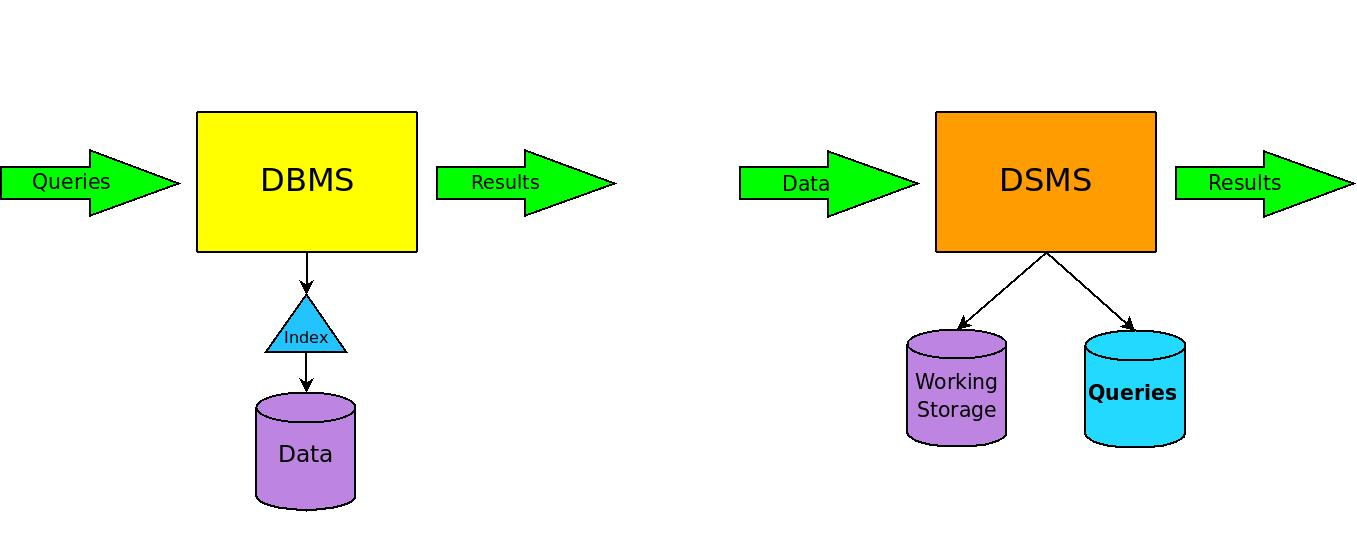
\includegraphics[width=\textwidth]{img/dbms+dsms}
	\caption{Comparison between a traditional Data Base Management System and a Data Stream Management System. On the
left queries are issued over stored data, while on the right data flows through continuous queries.}
	\label{fig:dbms+dsms}
\end{figure}

% %apps
% Data stream processing can be applied in many applications domains. Large scale scientific experiments, like particle
% accelerators~\cite{lhc} or radio telescopes~\cite{starglobe-grid}, produce a very large amount of data, which needs to be processed in real-time. 
% It also have found application in the area of large-scale supply chain management~\cite{hifi}. In order to keep track of the
% movements of items among warehouses, goods can be tagged with RFID chips and be scanned whenever entering or exiting a 
% storage location. Analysing these readings in real-time allows to keep an updated picture of the availability of goods
% at different locations and ultimately can lead to a great reduction in logistical costs.
% Financial data processing is also a major domain for DSMSs~\cite{streambase-algo}. Streams of data coming from the financial markets, for
% example tracking the value of a particular stock, can be processed in real-time to make better decisions about trades.
% In this case, the low-latency characteristics of DSMSs are particularly useful as being able to make a trade even split
% seconds before a competitor is key for maximum profitability.
% Sensor networks also provide a good application domain for stream processing~\cite{stream-processing-challanges, gsn0,
% senseweb}. These sensors produce a constant stream 
% of measurements which is well suited to be processed in a DSMS. Similarly, network monitoring is also a field in which
% stream processing can be successfully applied. In this case the data streams are not produced sensing the physical
% world, but instead monitor more ephemeral quantities describing how data packets move within a network. In this regard
% DSPSs can be employed to monitor the spreading of an worm or in general the health of the network~\cite{dec-net-mon,
% phi}.

\begin{comment}
\subsection{Data Models}
DSPSs are concerned with the processing of streams of data. These are possibly infinite sequences of timestamped
entities, called \textit{tuples}. By definition~\cite{dsm-issues} tuples in a data stream are: \textit{real-time,
continuous} and \textit{ordered}. Tuples in a stream are also characterised by a fixed relational schema, they are 
always composed by the same set of attributes. The nature of this attributes is really of no concerned for the model.
A data stream can represent a time series of measurements taken by a sensor, audio/video data, events and so on. 
A more formal definition of streams and query languages will be presented in Chapter~\ref{ch:language}.

Different approaches have been proposed for expressing queries over data streams. In the \textit{Boxes-and-Arrows}
model, operators are depicted as black boxes, joined together by arrows representing the data streams flowing through
them~\cite{aurora-and-medusa}. This is a very graphical and intuitive way of composing queries, even though it might become confusing when trying
to express particularly complex queries. \\
The de-facto standard in stream processing is to employ a more declarative approach. Building form the experience in
traditional databases, in this model the user describe the desired results through an SQL-based language. The system
then implements the query using a combination of processing operators and data streams flowing among them. This approach
is usually more intuitive for complex queries as it allow the user to focus on the nature of the results and not on the
query internal structure. The language used to express queries is usually CQL~\cite{cql} or one of its derivations like
StreamSQL~\cite{streamsql}. A more detailed discussion of the data models and these languages can be found in Chapter~\ref{ch:model}. 
\end{comment}

% \subsection{Approximate Processing}
% \label{sec:dsps-approx}
% Of particular interest for my research is the approximation techniques employed by these systems to cope with overload
% conditions. In a centralised DSPS all the computation is carried out by a single processing unit, so exploiting
% efficiently all the available resources is vital. 
% Resources are usually provisioned based on the average needs of the system, but the amount of needed resources can vary over time. 
% Even though these systems are designed with efficiency in mind, it is not uncommon for the system to run out of resources. 
% When that happen, the system has to resolve to \emph{approximate processing}.
% There are two primary reasons for which a DSMS may become
% overloaded: insufficient computing power or insufficient memory.
% 
% \textit{CPU-limited} overload is cause by an excessive rate of incoming tuples. In this situation, the system doesn't
% have enough computing power and there is insufficient CPU time to process all the elements in the input element. In this
% case the system can overcome the overload situation by discarding a subset of the incoming tuples. This technique of
% discarding a part of the input takes the name of \textit{load-shedding}. It has been shown in~\cite{load-shedding} that 
% for many applications it is acceptable to gracefully degrade the quality of the results, by providing approximate 
% processing during load spikes. If the statistical distribution of values in a stream is know, for instance by sampling,
% probabilistic guarantees on the accuracy of sliding-window aggregation queries can be derived
% mathematically~\cite{load-shedding-aggregate}.
% 
% 
% \textit{Memory-limited} overload occurs when the total state for all the registered queries exceeds the available
% memory. In this case, the system has to reduce the memory usage by reducing the state kept by operators. 
% In general the system will try to minimize its memory footprint as much as possible employing a number of techniques.
% For instance it can exploit constraints on streams to reduce state, either by letting the user specify them or by
% inferring them at run-time. It can also share state among operators when they materialize nearly identical relations.
% It can also schedule operators intelligently in order to minimize the length of queues in memory~\cite{stream-chains}.
% While these techniques do not lower the quality of the processing, sometimes the memory usage might still exceed the
% limits of the systems. In this situation, the internal state of operators can be approximated. In the case of
% aggregation and join operators, the state can be reduced by employing sampling techniques, like using
% \emph{histograms}~\cite{histograms}. These are approximations to datasets, achieved by partitioning the data into
% subsets, which are in turn summarised by an aggregate functions. Every column in the histogram is a compact
% representation of one of these subsets. Another summarising technique that can be employed makes use of
% wavelet synopses~\cite{wavelets}. For set difference, set intersection and duplicate
% elimination operators Bloom filters can be employed~\cite{approx-bloom}. These are compact set representation that allow
% a fast way of testing whether an element is a member of the set. All these techniques trade memory use against precision, but can
% greatly help the system in overcoming or avoiding memory-limited overload conditions.
% 
% In the scope of building our dependable stream processing system, all these approximation techniques can be useful. The
% main idea behind my work is that imperfect processing might still be meaningful in many contexts. In our system, when a
% node becomes overloaded, it will try to migrate some operators to another node. If no other node is available, or during
% the search phase, an overloaded node can employ these techniques to reduce its load and overcome the overload condition. 
% %systems
% \subsection{Research Prototypes}

\subsection*{STREAM}
\label{sec:stream}

STREAM~\cite{stream} is a centralised DSPS which tries to address the issue of long-running continuous queries. It
introduces a relational language called Continuous Query Language (CQL)~\cite{cql}, which allows the expression of
SQL-like queries over continuous data streams (Section~\ref{sec:cql}).  
Once a query is registered in the system, a correspondent \textit{query plan} is
compiled from it. Query plans are composed of \textit{operators}, which perform the actual processing, \textit{queues} which
buffer tuples as they move between operators, and \textit{synopses}, which store operator state. These elements are
composed to form a query plan implementing the CQL query. An example of query plan is depicted in Figure~\ref{fig:stream}. 
The incoming tuples are first stored in two sliding windows. Then they pass through two operators, first a \textsc{Join}
and then a \textsc{Select}. Synopsis are used by stateful operators to maintain some information about past tuples. In
between operators, tuples are always buffered using queues. Arrows represent data streams. 

\begin{figure}[b!]
	\centering
	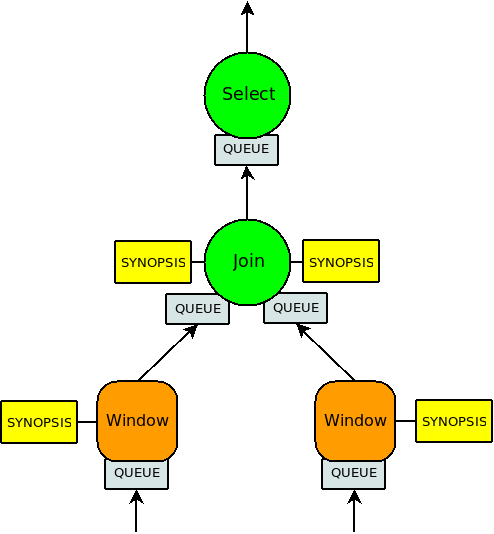
\includegraphics[width=0.5\textwidth]{img/stream.png} 
	\label{fig:stream}
	\caption{A simple query plan illustrating operators, queues, and synopses.} 
\end{figure} 

The major contribution of STREAM to the field is the introduction of CQL, that proved to be a very successful language. 
StreamSQL~\cite{streamsql}, an extension of CQL, is now considered the de-facto standard in stream processing.  

Being a centralised system, lacking the possibility to add resource to increase the processing capacity, STREAM made many
efforts to be as efficient as possible.  Within the engine massive stream and synopsis reuse is performed in order to
reduce the resource impact and maximise the number of queries executed on the node. Also some work has been done on the
scheduling of operators. While the first versions only included a round-robin policy, later a new algorithm called
\textit{chain scheduling}~\cite{stream-chains} has been introduced to minimize the memory footprint of the process. The
system also employs some approximations to deal with situation where the available resources are not sufficient to
support all the processing. In the event of overload, the system implements many approximation techniques to reduce the
quality of the results while continuing processing. STREAM also includes a graphical user interface which allow to
examine the query plan and to inspect the internal status of operators at run-time.

\paragraph{Considerations} 
STREAM has been a major contributor in the field of stream processing.
It introduced CQL, which allows the expression of complex queries with a simple declarative semantic, which become one
of the standards in the field of stream processing. I also plan to employ a declarative language in DISSP, an extension
of CQL, including the \emph{quality-metrics} described in Section~\ref{sec:metrics}.
STREAM also adopts several approximation techniques, to recover from CPU overload and memory shortage, like the ones described 
in Section~\ref{sec:dsps-approx}, which will be useful in the scope of my research.


\subsection*{HiFi}
\label{sec:hifi}

HiFi~\cite{hifi} is a system designed to manage large supply chains, monitoring the availability and location of goods
making use of RFID tags In the scope a national or international distribution network, keeping track of information
throughout the whole supply chain is a difficult task. Nevertheless, it is widely recognized that an accurate and
real-time monitoring of it can lead to great savings for a company. In this regard the envisioned solution is based on
RFID technology. Every product going in and out a warehouse is monitored and tracked. Because of its nature, RFID
technology is prone to errors. A tag might be scanned twice or not at all, and this poses even more burden on the
monitoring infrastructure. HiFi employs a number of techniques to minimise this error, like data cleaning, detection of
faulty receptors, conversion, calibration and so on. 

The architecture of HiFi is referred to as \emph{high fan}, in which a high number of sources generates data which is
hierarchically processed through successive aggregations, until it reaches the final user. Because of its shape this is
also called a ``bowtie'' system. The reasons for its peculiar configuration are due to two main reasons. First, a
flatter architecture would not be able to cope with the sheer amount of raw data produced by the sources.  Second, this
kind of structure is well suited for the tasks the system was designed for, which is mainly supply chain monitoring. In
this scenario, a company is likely to want to concentrate the final data processing and storage in a central private
facility, but it still needs to push some of the data cleaning, filtering and aggregation close to the input entry
points.  HiFi is built around TelegraphCQ\cite{telegraphcq} and TinyDB\cite{tinydb} It represent a custom solution to a
specific problem, even though its architecture could be suitable also for other purposes.

\paragraph{Considerations}
HiFi can be considered a centralised stream processing system, design for a specific application domanin.
It is built for large supply chain management, monitoring goods moving among warehouses with the use of RFID tags.
It suuports data cleaning, meaning the removal of spurious tag readings, in order to produce more accurate results.
In general, when working with sensor data, having a stage of data cleaning is a good idea. This idea could be
incorporated within the DISSP prototype, with a sanitising component located at entry points of the system.


%\subsection*{Aurora}
\label{sec:aurora}
\begin{structure}
	\item System Description
	\item Query Model
	\item A bit about Medusa
	\item Discsussion
\end{structure}

Aurora: \cite{aurora_and_medusa}


%\subsection*{NiagaraCQ}
\begin{structure}
	\item System Description
	\item Out-of-order processing
	\item Punctuation 
	\item Discsussion
\end{structure}

[NiagaraCQ] NiagaraCQ: A Scalable Continuous Query System for Internet Databases \cite{niagaracq}

[NiagaraST] Out-of-order processing: a new architecture for high-performance
stream systems \cite{out-of-order}

[NiagaraST] Exploiting Punctuation Semantics in Continuous Data Streams
\cite{punctuation-semantic}



%\subsection*{TelegraphCQ}
\begin{structure}
	\item System Description
	\item Discsussion
\end{structure}

TelegraphCQ~\cite{telegraphcq} is another centralised stream processing engine, which presents some original
architectural approaches. It builds on a previous work, called Telegraph and adds to it support for continuous queries.
Telegraph is composed by an extensible set of operators, or dataflow modules, that produce and consume records similarly
to ´´


\subsection*{XStream}
\label{sec:xstream}

\paragraph{Overview}
XStream~\cite{xstream} is a stream processing engine specifically designed to be employed in applications requiring the
processing of hight-rates data streams. Many classes of sensors are nowadays able to produce measurement
at a very high rate, sensing phenomena tens to hundreds of times per seconds. In particular it focuses on the efficient
processing of \textit{isochronous} data, or regularly sampled in time. Tuples in a data stream contain chunks of sampled
data, called \textit{signal segments} or SigSeg. These are a new abstract data type introduced by XStream and 
encapsulates a finite sequence of isochronous samples into an array-like data structure with associated timing metadata.
Because of this property of the data, per tuple timestamps are not necessary. SigSegs make it possible to pass windows
of data between operators as first class objects. This allows operators to not define their own input
windows as SigSegs already carry a window of data. SigSegs are very beneficial, for instance, in the scope of temporal
joins. These operators usually incur in a large computational overhead for large windows, due to the sheer number of
comparisons that must be made. XStream also introduce a new kind of scheduler, that dispatches tuples to operators in a
mostly depth-first traversal of the query plan. This also schedules SigSegs instead of single tuples, greately reducing
the overhead derived by the manipulation of a great number of individuals tuples. For specific applications dealing with
high-rate isochronous data, XStreams achieves incredible 1000x performace gains over traditional stream processing engines.

\paragraph{Considerations}
Differently than conventional stream processing engines which aim at being as general purpose as possible, XStreams is
optimized for a well defined class of input data, where tuples in a stream are separated by an equal amount of time. 
Because of this assumption on the incoming data streams, the system has been highly optimized and obtain an amazing
performance increase for some applications. The idea of employing array-like structure of isochronous data, or SigSegs,
as the basic computational unit is interesting, it is an optimization that could also be used by other DSPSs.



